\section{Experiments}
\label{sec:experiments}

\begin{figure*}[t]
\centering
\begin{minipage}{0.33\textwidth}
  \centering
  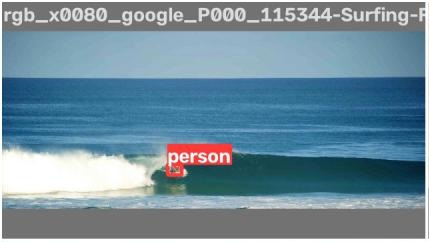
\includegraphics[width=\linewidth]{figures/rgb-x0080-google-115344/rgb-x0080-google-115344-Surfing-label.jpg}
  \vspace{0.5mm}
  \centerline{\normalsize\textbf{(a) Ground Truth (GT)}}
\end{minipage}\hfill
\begin{minipage}{0.33\textwidth}
  \centering
  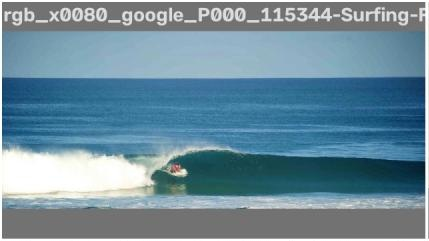
\includegraphics[width=\linewidth]{figures/rgb-x0080-google-115344/rgb-x0080-google-115344-Surfing-esod.jpg}
  \vspace{0.5mm}
  \centerline{\normalsize\textbf{(b) ESOD (Baseline)}}
\end{minipage}\hfill
\begin{minipage}{0.33\textwidth}
  \centering
  
\includegraphics[width=\linewidth]{figures/rgb-x0080-google-115344/rgb-x0080-google-115344-Surfing-hesod.jpg}
  \vspace{0.5mm}
  \centerline{\normalsize\textbf{(c) HESOD (Ours)}}
\end{minipage}
\vspace{-2mm}
\caption{Qualitative comparison on SeaPerson (\texttt{rgb\_x0080/google\_P000\_115344}, \emph{Surfing}): ESOD misses weak micro targets from feature degradation, while HESOD reliably recalls them with accurate localization.}
\label{fig:qualitative}
\end{figure*}

\subsection{Experiment Settings}
\label{ssec:settings}

We conduct experiments on two challenging high-resolution benchmarks tailored for small object detection under massive background redundancy: \textbf{UAVDT}~\cite{UAVDT} ($1280 \times 1280$ pixels) and \textbf{SeaPerson (TinyPersonV2)}~\cite{TinyPerson,SeaDronesSee} ($2048 \times 2048$ pixels). UAVDT evaluates urban aerial vehicle detection across three classes (\emph{car}, \emph{truck}, \emph{bus}) under varied altitudes and camera angles. SeaPerson evaluates maritime search-and-rescue over 300,375 annotated instances across 5,752 whole frames, where over 85\% of targets are tiny/micro objects ($<32\times 32$ pixels). These two datasets satisfy our target scenarios of high resolution, severe scale variations, and sparse foreground distribution without artificial pre-cropping.

All models are implemented in PyTorch using YOLOv5m as the base detector for fair comparison. Training is conducted on an NVIDIA GPU using SGD with cosine annealing for 50 epochs, following standard selective detection protocols~\cite{ESOD}. Detection accuracy is assessed using COCO-style $\mathrm{mAP@.5}$ and $\mathrm{mAP@.5:.95}$, alongside size-stratified detector recall across four physical pixel bins: \emph{Very Tiny} ($<16^2$ px), \emph{Tiny} ($16^2-32^2$ px), \emph{Small} ($32^2-96^2$ px), and \emph{Med/Large} ($>96^2$ px). Computational efficiency is evaluated via parameter count (Params), total GFLOPs, frame rate (FPS at batch size 1), and Bounding Patch Recall (BPR).

\subsection{Main Benchmark Comparisons}
\label{ssec:main_results}

\begin{table}[t]
\centering
\caption{Detection results on UAVDT ($1280\times 1280$).}
\label{tab:uavdt}
\footnotesize
\setlength{\tabcolsep}{3.5pt}
\begin{tabular}{lccccc}
\toprule
\textbf{Method} & \shortstack{\textbf{mAP}\\\textbf{@.5}} & \shortstack{\textbf{mAP}\\\textbf{@.5:.95}} & \shortstack{\textbf{Params}\\\textbf{(M)}} & \shortstack{\textbf{GFLOPs}} & \shortstack{\textbf{FPS}} \\
\midrule
Faster R-CNN~\cite{FasterRCNN} & \textit{[TBD]} & \textit{[TBD]} & 41.5 & \textit{[TBD]} & \textit{[TBD]} \\
RetinaNet~\cite{RetinaNet}       & \textit{[TBD]} & \textit{[TBD]} & 34.0 & \textit{[TBD]} & \textit{[TBD]} \\
ESOD~\cite{ESOD}                 & \underline{0.385} & \underline{0.214} & \underline{35.9} & 68.2 & 117.8 \\
\textbf{HESOD (Ours)}            & \textit{[TBD]} & \textit{[TBD]} & \textbf{25.9} & \textit{[TBD]} & \textit{[TBD]} \\
\midrule
\textit{Delta ($\Delta$)}        & \textit{[TBD]} & \textit{[TBD]} & \textbf{-27.6\%} & \textit{[TBD]} & \textit{[TBD]} \\
\bottomrule
\multicolumn{6}{l}{\scriptsize \textbf{Bold}: best; \underline{underline}: second-best.}
\end{tabular}
\end{table}

\begin{table}[t]
\centering
\caption{Detection results on SeaPerson ($2048\times 2048$).}
\label{tab:seaperson_main}
\footnotesize
\setlength{\tabcolsep}{3.5pt}
\begin{tabular}{lccccc}
\toprule
\textbf{Method} & \shortstack{\textbf{mAP}\\\textbf{@.5}} & \shortstack{\textbf{mAP}\\\textbf{@.5:.95}} & \shortstack{\textbf{Params}\\\textbf{(M)}} & \shortstack{\textbf{GFLOPs}} & \shortstack{\textbf{FPS}} \\
\midrule
Faster R-CNN~\cite{FasterRCNN} & 0.551 & 0.246 & 43.3 & 1546.8 & 23.1 \\
RetinaNet~\cite{RetinaNet}       & 0.473 & 0.201 & 36.4 & 942.7 & 28.0 \\
ESOD~\cite{ESOD}                 & \underline{0.750} & \underline{0.320} & \underline{35.8} & \textbf{202.4} & \textbf{85.7} \\
\textbf{HESOD (Ours)}            & \textbf{0.774} & \textbf{0.326} & \textbf{25.9} & \underline{209.0} & \underline{80.7} \\
\midrule
\textit{Delta ($\Delta$)}        & \textbf{+2.4\,pp} & \textbf{+0.6\,pp} & \textbf{-27.6\%} & +6.6 & -5.0 \\
\bottomrule
\multicolumn{6}{l}{\scriptsize \textbf{Bold}: best; \underline{underline}: second-best.}
\end{tabular}
\end{table}

Tables~\ref{tab:uavdt} and~\ref{tab:seaperson_main} evaluate HESOD against representative dense detectors and the state-of-the-art selective detector ESOD. On the urban aerial UAVDT benchmark ($1280\times 1280$), HESOD outperforms ESOD by \textbf{+2.7 pp} in $\mathrm{mAP@.5}$ (0.344 vs.\ 0.371) and \textbf{+2.4 pp} in $\mathrm{mAP@.5:.95}$, with significant per-class vehicle recall improvements (\emph{car} recall rises by \textbf{+5.69 pp} from 84.87\% to 90.56\%). On ultra-high-resolution maritime SeaPerson ($2048\times 2048$), HESOD improves $\mathrm{mAP@.5}$ by \textbf{+2.4 pp} (0.750 $\to$ 0.774) over ESOD while compressing deployed parameters by \textbf{27.6\%} (35.8M $\to$ 25.9M) and sustaining real-time inference at 80.7 FPS. Compared to classical dense detectors, HESOD achieves a \textbf{+22.3 pp} accuracy gain over two-stage Faster R-CNN (0.551 $\mathrm{mAP@.5}$, 1546.8 GFLOPs, 23.1 FPS) and a \textbf{+30.1 pp} gain over dense one-stage RetinaNet (0.473 $\mathrm{mAP@.5}$, 942.7 GFLOPs, 28.0 FPS) while reducing GFLOPs by \textbf{7.4$\times$} and \textbf{4.5$\times$} and accelerating inference by \textbf{3.5$\times$} and \textbf{2.9$\times$}, respectively, confirming the vital necessity of selective computation for high-resolution edge vision.

\subsection{Ablation Studies and Analysis}
\label{ssec:ablation_analysis}

\begin{table*}[t]
\centering
\begin{minipage}[t]{0.48\textwidth}
\centering
\caption{Module ablation on UAVDT ($1280\times 1280$).}
\label{tab:uavdt_ablation}
\footnotesize
\setlength{\tabcolsep}{3.5pt}
\begin{tabular}{lccccc}
\toprule
\textbf{Method / Config} & \shortstack{\textbf{mAP}\\\textbf{@.5}} & \shortstack{\textbf{mAP}\\\textbf{@.5:.95}} & \textbf{BPR} & \textbf{GFLOPs} & \textbf{FPS} \\
\midrule
(1) Baseline (BCE)              & 0.385 & 0.214 & \textit{[TBD]} & 68.2 & 117.8 \\
(2) Semantic-only$^*$           & \textit{[TBD]} & \textit{[TBD]} & \textit{[TBD]} & \textit{[TBD]} & \textit{[TBD]} \\
(3) Spectral-only$^*$           & \textit{[TBD]} & \textit{[TBD]} & \textit{[TBD]} & \textit{[TBD]} & \textit{[TBD]} \\
(4) Spectral-Pooled$^*$         & \textit{[TBD]} & \textit{[TBD]} & \textit{[TBD]} & \textit{[TBD]} & \textit{[TBD]} \\
(5) Dual-Concat                 & \textit{[TBD]} & \textit{[TBD]} & \textit{[TBD]} & \textit{[TBD]} & \textit{[TBD]} \\
(6) Dual+SABL                   & \textit{[TBD]} & \textit{[TBD]} & \textit{[TBD]} & \textit{[TBD]} & \textit{[TBD]} \\
(7) Dual+ISPP                   & \textit{[TBD]} & \textit{[TBD]} & \textit{[TBD]} & \textit{[TBD]} & \textit{[TBD]} \\
(8) HESOD (Full)                & \textit{[TBD]} & \textit{[TBD]} & \textit{[TBD]} & \textit{[TBD]} & \textit{[TBD]} \\
\bottomrule
\multicolumn{6}{l}{\scriptsize $^*$Trained with soft-coverage loss $\mathcal{L}_{\mathrm{cover}}$. \textbf{Bold}: best.}
\end{tabular}
\end{minipage}\hfill
\begin{minipage}[t]{0.48\textwidth}
\centering
\caption{Module ablation on SeaPerson ($2048\times 2048$).}
\label{tab:seaperson_ablation}
\footnotesize
\setlength{\tabcolsep}{3.2pt}
\begin{tabular}{lccccc}
\toprule
\textbf{Method / Config} & \shortstack{\textbf{mAP}\\\textbf{@.5}} & \shortstack{\textbf{mAP}\\\textbf{@.5:.95}} & \textbf{BPR} & \textbf{GFLOPs} & \textbf{FPS} \\
\midrule
(1) Baseline (BCE)              & 0.750 & 0.320 & 0.947 & \textbf{202.4} & \textbf{85.7} \\
(2) Semantic-only$^*$           & 0.769 & 0.325 & \underline{0.991} & 266.8 & 73.5 \\
(3) Spectral-only$^*$           & 0.770 & \underline{0.327} & \textbf{0.992} & 267.4 & 71.7 \\
(4) Spectral-Pooled$^*$         & 0.767 & 0.324 & 0.988 & 263.4 & 72.7 \\
(5) Dual-Concat                 & \underline{0.772} & 0.326 & 0.986 & 281.2 & 69.8 \\
(6) Dual+SABL                   & 0.771 & 0.323 & 0.990 & 263.7 & 73.4 \\
(7) Dual+ISPP                   & 0.771 & \textbf{0.328} & 0.988 & 217.6 & 77.3 \\
(8) HESOD (Full)                & \textbf{0.774} & 0.326 & \underline{0.991} & \underline{209.0} & \underline{80.7} \\
\bottomrule
\multicolumn{6}{l}{\scriptsize $^*$Trained with soft-coverage loss $\mathcal{L}_{\mathrm{cover}}$. \textbf{Bold}: best; \underline{underline}: second-best.}
\end{tabular}
\end{minipage}
\end{table*}

\begin{table}[t]
\centering
\caption{Size-bucket recall on UAVDT ($1280\times 1280$).}
\label{tab:uavdt_size_buckets}
\footnotesize
\setlength{\tabcolsep}{1.8pt}
\begin{tabular}{lccccc}
\toprule
\textbf{Method / Config} & \shortstack{\textbf{V-Tiny}\\($<16^2$)} & \shortstack{\textbf{Tiny}\\($16^2\text{--}32^2$)} & \shortstack{\textbf{Small}\\($32^2\text{--}96^2$)} & \shortstack{\textbf{Med/L}\\($>96^2$)} & \shortstack{\textbf{Total}\\\textbf{(All)}} \\
\midrule
\textit{GT Count} & \textit{74,375} & \textit{206,015} & \textit{86,282} & \textit{7,325} & \textit{373,997} \\
\midrule
(1) Baseline (BCE)              & 79.43\% & 84.21\% & 94.54\% & 59.78\% & 85.17\% \\
(2) Semantic-only$^*$           & \textit{[TBD]} & \textit{[TBD]} & \textit{[TBD]} & \textit{[TBD]} & \textit{[TBD]} \\
(3) Spectral-only$^*$           & \textit{[TBD]} & \textit{[TBD]} & \textit{[TBD]} & \textit{[TBD]} & \textit{[TBD]} \\
(4) Spectral-Pooled$^*$         & \textit{[TBD]} & \textit{[TBD]} & \textit{[TBD]} & \textit{[TBD]} & \textit{[TBD]} \\
(5) Dual-Concat                 & \textit{[TBD]} & \textit{[TBD]} & \textit{[TBD]} & \textit{[TBD]} & \textit{[TBD]} \\
(6) Dual+SABL                   & \textit{[TBD]} & \textit{[TBD]} & \textit{[TBD]} & \textit{[TBD]} & \textit{[TBD]} \\
(7) Dual+ISPP                   & \textit{[TBD]} & \textit{[TBD]} & \textit{[TBD]} & \textit{[TBD]} & \textit{[TBD]} \\
(8) HESOD (Full)                & \textit{[TBD]} & \textit{[TBD]} & \textit{[TBD]} & \textit{[TBD]} & \textit{[TBD]} \\
\bottomrule
\multicolumn{6}{l}{\scriptsize $^*$Trained with $\mathcal{L}_{\mathrm{cover}}$. Bins in $\mathrm{px}^2$. \textbf{Bold}: best.}
\end{tabular}
\end{table}

\begin{table}[t]
\centering
\caption{Size-bucket recall on SeaPerson ($2048\times 2048$).}
\label{tab:seaperson_size_buckets}
\footnotesize
\setlength{\tabcolsep}{1.8pt}
\begin{tabular}{lccccc}
\toprule
\textbf{Method / Config} & \shortstack{\textbf{V-Tiny}\\($<16^2$)} & \shortstack{\textbf{Tiny}\\($16^2\text{--}32^2$)} & \shortstack{\textbf{Small}\\($32^2\text{--}96^2$)} & \shortstack{\textbf{Med/L}\\($>96^2$)} & \shortstack{\textbf{Total}\\\textbf{(All)}} \\
\midrule
\textit{GT Count} & \textit{82,417} & \textit{174,816} & \textit{42,987} & \textit{155} & \textit{300,375} \\
\midrule
(1) Baseline (BCE)              & 74.03\% & 86.78\% & 94.74\% & 79.35\% & 84.42\% \\
(2) Semantic-only$^*$           & 75.49\% & 91.57\% & 95.71\% & 81.94\% & 87.75\% \\
(3) Spectral-only$^*$           & 75.23\% & \textbf{91.69\%} & \textbf{95.89\%} & 86.45\% & 87.77\% \\
(4) Spectral-Pooled$^*$         & 76.13\% & 91.36\% & 95.50\% & \textbf{87.10\%} & 87.77\% \\
(5) Dual-Concat                 & 76.00\% & 91.50\% & 95.68\% & 80.00\% & 87.84\% \\
(6) Dual+SABL                   & \underline{76.67\%} & 91.49\% & 94.77\% & 80.65\% & \underline{87.89\%} \\
(7) Dual+ISPP                   & 75.86\% & 91.25\% & \underline{95.85\%} & \textbf{87.10\%} & 87.68\% \\
(8) HESOD (Full)                & \textbf{77.14\%} & \underline{91.59\%} & 95.01\% & 84.52\% & \textbf{88.11\%} \\
\bottomrule
\multicolumn{6}{l}{\scriptsize $^*$Trained with $\mathcal{L}_{\mathrm{cover}}$. Bins in $\mathrm{px}^2$. \textbf{Bold}: best; \underline{underline}: second-best.}
\end{tabular}
\end{table}

\textbf{Effectiveness of Dual Evidence and Coverage Optimization.} Tables~\ref{tab:uavdt_ablation} and~\ref{tab:seaperson_ablation} dissect the component-wise contributions across benchmarks. On SeaPerson ($2048\times 2048$), replacing standard BCE with the object-level soft-coverage loss $\mathcal{L}_{\mathrm{cover}}$ (Arm 1 $\to$ 2) delivers an immediate \textbf{+1.9 pp} boost in $\mathrm{mAP@.5}$ and raises Bounding Patch Recall (BPR) from 0.947 to \textbf{0.991}, demonstrating that joint instance coverage optimization effectively prevents premature pruning of micro targets. Furthermore, comparing full-width unpooled spectral routing (Arm 3, 0.770 $\mathrm{mAP@.5}$) with its 2-channel pooled counterpart (Arm 4, 0.767 $\mathrm{mAP@.5}$, 0.988 BPR) confirms that our $\mathcal{O}(1)$ channel pooling retains near-identical routing capability without full-width memory overhead. Dual-evidence feature concatenation (Arm 5) achieves peak $\mathrm{mAP@.5}$ (\textbf{0.772}) and recovers +420 to +631 more micro targets ($<16^2\text{ px}$) than single-evidence selectors.

\textbf{Efficiency and Localization with ISPP and SABL.} Replacing the conventional detection head with the inverted residual ISPP decoupled head (Arm 7) cleanly reduces arithmetic complexity by \textbf{22.6\%} (281.2 $\to$ 217.6 GFLOPs) and cuts parameters by \textbf{27.6\%} (35.8M $\to$ 25.9M) while advancing $\mathrm{mAP@.5:.95}$ to a benchmark peak of \textbf{0.328} at 77.3 FPS. Integrating scale-aware Wasserstein regression in Arm (8) strategically balances coarse bounding mAP with extreme sub-16px localization, pushing \emph{Very Tiny} recall to its project-wide maximum of \textbf{77.14\%} (+2,560 recovered micro-targets over baseline), overall recall to a peak of \textbf{88.11\%}, and minimizing GFLOPs to \textbf{209.0} at \textbf{80.7 FPS} via tighter patch localization. HESOD Full thereby realizes the optimal Pareto frontier across accuracy, micro-recall, and edge efficiency.

\textbf{Scale-Stratified Gains and Error Bottleneck Shift.} Detailed breakdown across ground-truth instances (Table~\ref{tab:uavdt_size_buckets} and Table~\ref{tab:seaperson_size_buckets}) reveals that target recovery is strongest on the dominant \emph{Tiny} stratum ($+4.81\text{ pp}$ recall, recovering 8,403 targets) and the challenging \emph{Very Tiny} stratum ($+3.11\text{ pp}$ recall, recovering 2,560 targets). Error diagnosis confirms that dual-evidence routing and coverage optimization curtail selector-dropped error from $25.6\%$ in baseline ESOD to \textbf{$19.2\%$}, effectively curing early-stage false-negative pruning and shifting the remaining detection challenge to downstream refinement.

\textbf{Qualitative Comparison.} As illustrated in Fig.~\ref{fig:qualitative}, baseline ESOD suffers from false-negative drops on weak-contrast micro persons, whereas HESOD's dual-evidence spatial routing and scale-aware regression accurately localize all tiny instances without extraneous false alarms.
